\fancychapter{A Simple and Effective Approach to Automatic Post-Editing with Transfer Learning}
\label{cap:ape}

In the following chapter, we will focus on this thesis' goal of
paving the way for more \textbf{data efficient} models. In order to
achieve this, we use weak supervion in the form of transfer learning.

When the article shown in this chapter was published, the use of
pre-trained transformers % TODO: refer this section in background
in NLP in generation tasks had not been explored as much as it has
been in recent years. % TODO: may cite T5 as an example of seq2seq
For instance, the work that proposed
BERT~\citep{devlin2018bert} had only been recently released and NLP
researchers were quickly interested in using it in a variety of
tasks. However, as BERT and other similar models were transformer
encoders, it was not straightforward to consider them to be used
as a sequence-to-sequence model. % TODO: refer this section in background

In this work, we presented a simple and effective
solution to this problem, using the scarcity of Automatic Post-Editing
data as the playground to explore the transfer learning capacity of
large transformer encoder models in a sequence-to-sequence task,
being one of the first works to do so.

\emph{This chapter is based on \citet{Correia2019}.}

\section{Motivation}

 {\bf Automatic post-editing}~\citep[APE;][]{simard2007rule} is
inspired by human post-editing, in which a translator corrects
mistakes made by an MT system.
The goal of APE is to automatically correct the mistakes produced by
a black-box MT system. APE is particularly
appealing for rapidly customizing MT, avoiding to train new systems
from scratch. Interfaces where human translators can post-edit and
improve the quality of MT
sentences~\citep{Alabau2014,Federico2014,Denkowski2015,Hokamp2018}
are a common data source for APE models, since they provide {\bf
    triplets} of {\it source} sentences ({\tt src}), {\it machine
    translation} outputs ({\tt mt}), and {\it human post-edits} ({\tt
    pe}).

Unfortunately, human post-edits are typically scarce. Existing APE
systems circumvent this by generating {\bf artificial
    triplets}~\citep{junczys2016log, negri2018escape}. However, this
requires access to a high quality MT system, similar to (or better
than) the one used in the black-box MT itself. This spoils the
motivation of APE as an alternative to large-scale MT training in the
first place: the time to train MT systems in order to extract these
artificial triplets, combined with the time to train an APE system on
the resulting large dataset, may well exceed the time to train a MT
system from scratch.

When the current work was published, the state of the art in APE used
a Transformer~\citep{vaswani2017attention} with {\bf two encoders},
for the {\tt src} and {\tt mt}, and {\bf one decoder}, for {\tt pe}.
This system was named the Dual-Source
Transformer~\citep{junczys2018ms, tebbifakhr2018multi}. When
concatenating human post-edited data and artificial triplets, these
systems greatly improved the MT baseline. However, little successes
are known using only the true data created by the human post-editors.

Meanwhile, there have been many successes of {\bf transfer learning}
for NLP: models such as CoVe~\citep{mccann2017learned},
ELMo~\citep{peters2018deep}, OpenAI GPT~\citep{radford2018improving},
ULMFiT~\citep{howard2018universal}, and BERT~\citep{devlin2018bert}
obtain powerful representations by training large-scale language
models and use them to improve performance in many sentence-level and
word-level tasks. However, a language generation task such as APE
presents additional challenges.

In this chapter, we build upon the successes above and show that {\bf
    transfer learning is an effective and time-efficient strategy for
    APE}, using a pre-trained BERT model. This is an appealing strategy
in practice: while large language models like BERT are expensive to
train, this step is only done once and covers many languages,
reducing engineering efforts substantially. This is in contrast with
the computational and time resources that creating artificial
triplets for APE needs---these triplets need to be created separately
for every language pair that one wishes to train an APE system for.

By contrast, using transfer learning and with only the small shared
task dataset (23K triplets), our proposed strategy outperforms this
baseline considerably, by $-$4.9 TER and $+$7.4 BLEU in the
English-German WMT 2018 APE shared task, with 3 hours of training on
a single GPU. Adding the artificial eSCAPE
dataset~\citep{negri2018escape} leads to a performance of 17.15 TER,
a new state of the art.

Our main contributions are the following:
\begin{itemize}
  \item We combine the ability of BERT to
        handle {\bf sentence pair inputs} together with its pre-trained
        multilingual model, to use both the {\tt src} and {\tt mt} in a
          {\bf cross-lingual encoder}, that takes a multilingual
        sentence pair as input.
  \item We show how pre-trained BERT models can also be used and
        fine-tuned as the {\bf decoder} in a language generation task.
  \item We make a thorough empirical evaluation of different ways of
        coupling BERT models in an APE system, comparing different options
        of parameter sharing, initialization, and fine-tuning.
\end{itemize}

\section{Previous Work}

In their Dual-Source Transformer model, \citet{junczys2018ms} also
found gains by tying together encoder parameters, and the embeddings
of both encoders and decoder. Our work confirms this but shows
further gains by using segment embeddings and more careful sharing
and initialization strategies. \citet{sachan2018parameter} explore
parameter sharing between Transformer layers. However, they focus on
sharing decoder parameters in a \emph{one-to-many} multilingual MT
system. In our work, we share parameters between the encoder and the
decoder.

As stated in \secref{sec:experiments}, \citet{berard2017lig} also
showed improved results over the MT baseline, using exclusively the
shared task data. Their system outputs edit operations that decide
whether to insert, keep or delete tokens from the machine translated
sentence. Instead of relying on edit operations, our approach
mitigates the small amount of data with transfer learning through
BERT.

Our work makes use of the recent advances in transfer learning for
NLP~\citep{peters2018deep, howard2018universal, radford2018improving,
  devlin2018bert}. Pre-training these large language models has largely
improved the state of the art of the GLUE
benchmark~\citep{wang2018glue}. Particularly, our work uses the BERT
pre-trained model and makes use of the representations obtained not
only in the encoder but also on the decoder in a language generation
task.

More closely related to our work, \citet{lample2019cross}
pre-trained a BERT-like language model using parallel data, which
they used to initialize the encoder and decoder for supervised and
unsupervised MT systems. They also used segment embeddings (along
with word and position embeddings) to differentiate between a pair of
sentences in different languages. However, this is only used in one
of the pre-training phases of the language model (translation
language modelling) and not in the downstream task. In our work, we
use segment embeddings during the downstream task itself, which is a
perfect fit to the APE task.

\section{Automatic Post-Editing with BERT}\label{sec:ape_bert}

\subsection{BERT as a Cross-Lingual Encoder}

Our transfer learning approach is based on the Bidirectional Encoder
Representations from Transformers~\citep[BERT;][]{devlin2018bert}.
This model obtains deep bidirectional representations by training a
Transformer~\citep{vaswani2017attention} with a large-scale dataset
in a masked language modeling task where the objective is to predict
missing words in a sentence. We use the BERT\textsubscript{BASE}
model, which is composed of $L=12$ self-attention layers, hidden size
$H=768$, $A=12$ attention heads, and feed-forward inner layer size
$F=3072$. In addition to the word and learned position embeddings,
BERT also has {\bf segment embeddings} to differentiate between a
segment A and a segment B---this is useful for tasks such as natural
language inference, which involve two sentences. In the case of APE,
there is also a pair of input sentences ({\tt src}, {\tt mt}) which
are in different languages. Since one of the released BERT models was
jointly pre-trained on 104 languages,\footnote{
  \url{https://github.com/google-research/bert/blob/master/multilingual.md}}
we use this multilingual BERT pre-trained model to encode the
bilingual input pair of APE.

Therefore, the whole encoder of our APE model is the multilingual
BERT: we encode both {\tt src} and {\tt mt} in the same encoder and
use the segment embeddings to differentiate between languages
(\figref{fig:transformer_diagram}). We reset positional
embeddings when the {\tt mt} starts, since it is not a continuation
of {\tt src}.

\begin{figure}[ht!]
  \centering
  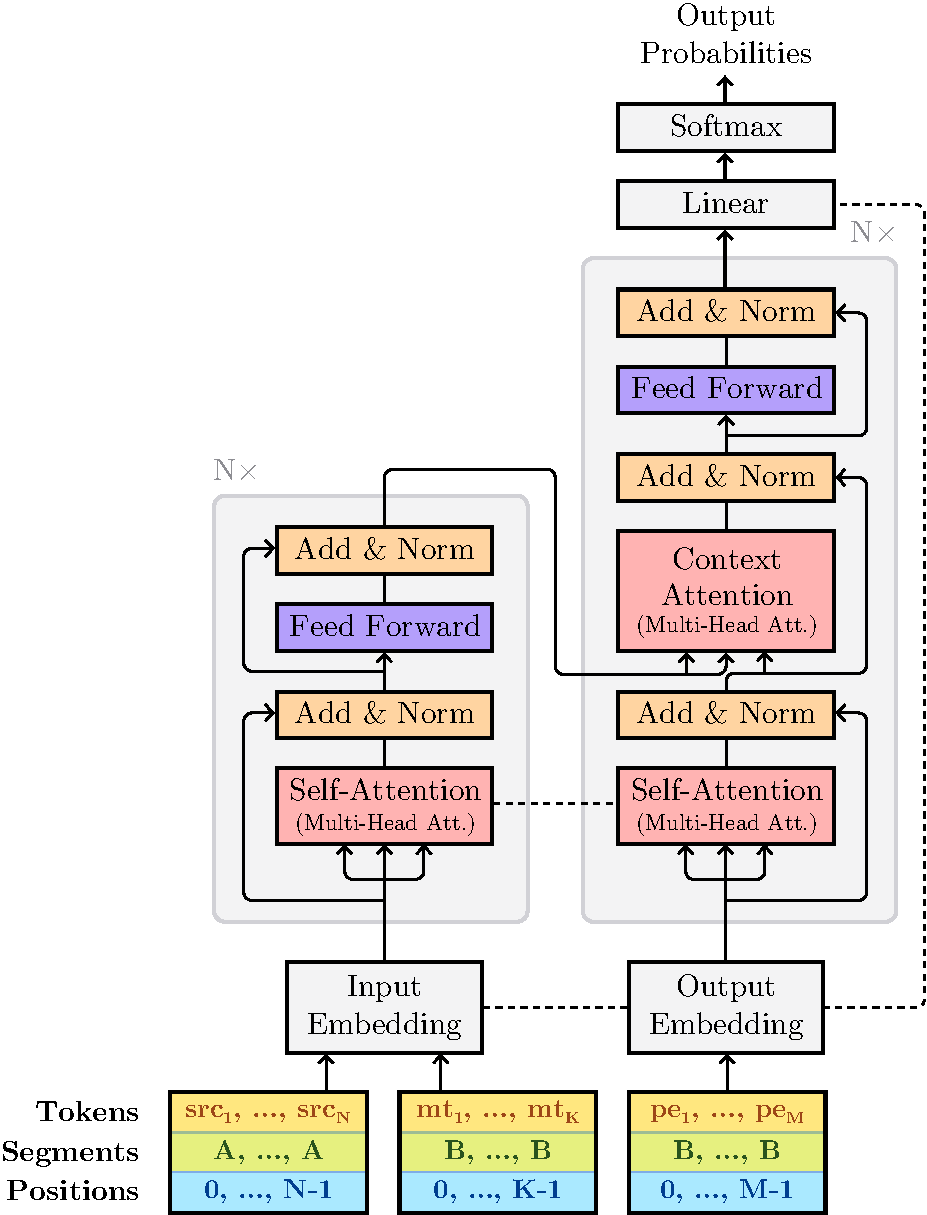
\includegraphics[width=0.9\textwidth]{Figures/bert-ape-diagram.pdf}
  \caption{\textbf{Dual-Source BERT.}
    Dashed lines show shared parameters in our best configuration.}
  \label{fig:transformer_diagram}
\end{figure}

\subsection{BERT as a Decoder}\label{sec:ape_bert_decoder}

Prior work has incorporated pre-trained models in {\it encoders}, but
not as {\bf decoders} of sequence-to-sequence models. Doing so
requires a strategy for generating fluently from the pre-trained
model. Note that the bidirectionality of BERT is lost, since the
model cannot look at words that have not been generated yet, and it
is an open question how to learn decoder-specific blocks (e.g.
context attention), which are absent in the pre-trained model.

One of our key contributions is to use BERT in the decoder by
experimenting different strategies for initializing and sharing the
self and context attention layers and the positionwise feed-forward
layers. We tie together the encoder and decoder embeddings weights
(word, position, and segment) along with the decoder output layer
(transpose of the word embedding layer). We use the same segment
embedding for the target sentence ({\tt pe}) and the second sentence
in the encoder ({\tt mt}) since they are in the same language. The
full architecture is shown in \figref{fig:transformer_diagram}.
We experiment with the following strategies for coupling BERT
pre-trained models in the decoder:

\begin{itemize}
  \item \textbf{Transformer.} A Transformer decoder as described in
        \citet{vaswani2017attention} without any shared parameters,
        with the BERT\textsubscript{BASE} dimensions and randomly
        initialized weights.
  \item \textbf{Pre-trained BERT.} This initializes the decoder with
        the pre-trained BERT model. The only component initialized randomly
        is the context attention (CA) layer, which is absent in BERT. Unlike
        in the original BERT model---which only encodes sentences---a mask in
        the self-attention is required to prevent the model from looking to
        subsequent tokens in the target sentence.
  \item \textbf{ BERT initialized context attention.} Instead of a
        random initialization, we initialize the context attention layers
        with the weights of the corresponding BERT self-attention layers.
  \item \textbf{Shared self-attention}. Instead of just having the same
        initialization, the self-attentions (SA) in the encoder and decoder
        are tied during training.
  \item \textbf{Context attention shared with self-attention.} We take
        a step further and \emph{tie} the context attention and self
        attention weights---making all the attention transformation matrices
        (self and context) in the encoder and decoder tied.
  \item \textbf{Shared feed-forward.} We tie the feed-forward weights
        (FF) between the encoder and decoder.
\end{itemize}

\section{Experiments} \label{sec:experiments}

We now describe our experimental results. Our models were implemented
on a fork of OpenNMT-py~\citep{klein2017opennmt} using a
Pytorch~\citep{pytorch} re-implementation of
BERT.\footnote{\url{https://github.com/huggingface/transformers}}
Our model's implementation is publicly
available.\footnote{\url{https://github.com/deep-spin/OpenNMT-APE}}

\paragraph*{Datasets.}
We use the data from the WMT 2018 APE shared
task~\citep{Chatterjee2018} (English-German SMT), which consists of
23,000 triplets for training, 1,000 for validation, and 2,000 for
testing. In some of our experiments, we also use the eSCAPE
corpus~\citep{negri2018escape}, which comprises about 8M sentences;
when doing so, we oversample 35x the shared task data to cover $10\%$
of the final training data. We segment words with
WordPiece~\citep{wu2016google}, with the same vocabulary used in the
Multilingual BERT. At training time, we discard triplets with 200+
tokens in the combination of {\tt src} and {\tt mt} or 100+ tokens in
  {\tt pe}. For evaluation, we use TER~\citep{snover2006study} and
tokenized BLEU~\citep{papineni2002bleu}.

\paragraph*{Training Details.}
We use Adam~\citep{kingma2014adam} with a triangular learning rate
schedule that increases linearly during the first 5,000 steps until
$5\times 10^{-5}$ and has a linear decay afterwards. When using BERT
components, we use a $\ell_2$ weight decay of $0.01$. We apply
dropout~\citep{srivastava2014dropout} with $p_{drop}=0.1$ to all
layers and use label smoothing with
$\epsilon=0.1$~\citep{pereyra2017regularizing}. For the small data
experiments, we use a batch size of 1024 tokens and save checkpoints
every 1,000 steps; when using the eSCAPE corpus, we increase this to
2048 tokens and 10,000 steps. The checkpoints are created with the
exponential moving average strategy of \citet{junczys2018marian}
with a decay of $10^{-4}$. At test time, we select the model with
best TER on the development set, and apply beam search with a beam
size of 8 and average length penalty.

\paragraph*{Initialization and Parameter Sharing.}
\tableref{tab:ablation_smt} compares the different decoder
strategies described in \secref{sec:ape_bert_decoder} on the WMT 2018
validation set. The best results were achieved by sharing the
self-attention between encoder and decoder, and by initializing (but
not sharing) the context attention with the same weights as the
self-attention. Regarding the self-attention sharing, we hypothesize
that its benefits are due to both encoder and decoder sharing a
common language in their input (in the {\tt mt} and {\tt pe}
sentence, respectively). Future work will investigate if this is
still beneficial when the source and target languages are less
similar. On the other hand, the initialization of the context
attention with BERT's self-attention weights is essential to reap the
benefits of BERT representations in the decoder---without it, using
BERT decreases performance when compared to a regular transformer
decoder. This might be due to the fact that context attention and
self-attention share the same neural block architecture (multi-head
attention) and thus the context attention benefits from the
pre-trained BERT's better weight initialization. No benefit was
observed from sharing the feed-forward weights.

\begin{table}[t]
  \centering
  \begin{tabular}{lcc}
    \toprule
                                                       & TER$\downarrow$ & BLEU$\uparrow$ \\
    \midrule
    Transformer decoder                                & 20.33           & 69.31          \\
    Pre-trained BERT                                   & 20.83           & 69.11          \\
    \hspace{1ex}\textcolor{gray}{\textit{with}}
    CA $\leftarrow$ SA                                 & 18.91           & 71.81          \\
    \textover[r]
    {\hspace{1ex}\textcolor{gray}{\textit{and}}}{\hspace{1ex}\textit{with}}
    \textover[r]
    {SA $\leftrightarrow$}
    {CA $\leftarrow$} Encoder SA                       & \textbf{18.44}  & \textbf{72.25} \\
    \textover[r]
    {\hspace{1ex}\textcolor{gray}{\textit{and}}}{\hspace{1ex}\textit{with}}
    \textover[r]
    {CA $\leftrightarrow$}{CA $\leftarrow$} SA         & 18.75           & 71.83          \\
    \textover[r]
    {\hspace{1ex}\textcolor{gray}{\textit{and}}}{\hspace{1ex}\textit{with}}
    \textover[r]
    {FF $\leftrightarrow$}{CA $\leftarrow$} Encoder FF & 19.04           & 71.53          \\
    \bottomrule
  \end{tabular}
  \caption{
    Ablation study of decoder configurations, by gradually having more
    shared parameters between the encoder and decoder (trained without
    synthetic data). $\leftrightarrow$ denotes parameter tying and
    $\leftarrow$ an initialization.
  }
  \label{tab:ablation_smt}
\end{table}

\paragraph*{Final Results.}
Finally, \tableref{tab:results_smt} shows our results on the WMT
2016--18 test sets. The model named \emph{BERT Enc.\,+\,BERT Dec.}
corresponds to the best setting found in
\tableref{tab:ablation_smt}, while \emph{BERT Enc.\,+\,Transformer
  Dec.} only uses BERT in the encoder. We show results for single
models and ensembles of 4 independent models.

Using the small shared task dataset only (23K triplets), our single
\emph{BERT Enc.\,+\,BERT Dec.} model surpasses the MT baseline by a
large margin ($-$4.90 TER in test 2018). The only system we are aware
to beat the MT baseline with only the shared task data is
\citet{berard2017lig}, which we also outperform ($-$4.05 TER in test
2017). With only about 3 GPU-hours and on a much smaller dataset, our
model reaches a performance that is comparable to an ensemble of the
best WMT 2018 system with an artificial dataset of 5M triplets
($+$0.02 TER in test 2016), which is much more expensive to train.
With 4$\times$ ensembling, we get competitive results with systems
trained on 8M triplets.

When adding the eSCAPE corpus (8M triplets), performance surpasses
the state of the art in all test sets. By ensembling, we improve even
further, achieving a final 17.15 TER score in test 2018 ($-$0.85 TER
than the previous state of the art).

\begin{landscape}
  \begin{table*}[t]
    \centering
    \begin{tabular}{lccccccc}
      \toprule
                                                       &                & \multicolumn{2}{c}{test 2016} &
      \multicolumn{2}{c}{test 2017}                    &
      \multicolumn{2}{c}{test 2018}                                                                                                      \\
      \cmidrule{3-4} \cmidrule{5-6}  \cmidrule{7-8}
      Model                                            & Train Size     & TER$\downarrow$               & BLEU$\uparrow$ &
      TER$\downarrow$                                  & BLEU$\uparrow$ & TER$\downarrow$               & BLEU$\uparrow$                 \\
      \midrule
      MT baseline (Uncorrected)                        &                &
      24.76                                            & 62.11          & 24.48                         & 62.49          & 24.24 & 62.99 \\
      \midrule
      \citet{berard2017lig}                            &
      \multicolumn{1}{c}{23K}                          &
      22.89                                            & ---            & 23.08                         & 65.57          & ---   & ---   \\
      \midrule
      \citet{junczys2018ms}                            &
      \multicolumn{1}{c}{\multirow{2}{*}{5M}}          &
      18.92                                            & 70.86          & 19.49                         & 69.72          & ---   & ---   \\
      \citet{junczys2018ms}$\times 4$                  &
      \multicolumn{1}{c}{}                             &
      18.86                                            & 71.04          & 19.03                         & 70.46          & ---   & ---   \\
      \midrule
      \citet{tebbifakhr2018multi}                      &
      \multicolumn{1}{c}{\multirow{3}{*}{8M}}          &
      ---                                              & ---            & ---                           & ---            & 18.62 & 71.04 \\
      \citet{junczys2018ms}                            &
      \multicolumn{1}{c}{}                             &
      17.81                                            & 72.79          & 18.10                         & 71.72          & ---   & ---   \\
      \citet{junczys2018ms}$\times 4$                  &
      \multicolumn{1}{c}{}                             &
      17.34                                            & 73.43          & 17.47                         & 72.84          & 18.00 & 72.52 \\
      \midrule
      \midrule
      Dual-Source Transformer$^\dagger$                &
      \multicolumn{1}{c}{\multirow{4}{*}{23K}}         &
      27.80                                            & 60.76          & 27.73                         & 59.78          & 28.00 & 59.98 \\
      BERT Enc.\,+\,Transformer Dec. (\emph{Ours})     &
      \multicolumn{1}{c}{}                             &
      20.23                                            & 68.98          & 21.02                         & 67.47          & 20.93 & 67.60 \\
      BERT Enc.\,+\,BERT Dec. (\emph{Ours})            &
      \multicolumn{1}{c}{}                             &
      18.88                                            & 71.61          & 19.03                         & 70.66          & 19.34 & 70.41 \\
      BERT Enc.\,+\,BERT Dec. $\times 4$ (\emph{Ours}) &
      \multicolumn{1}{c}{}                             &
      \textbf{18.05}                                   & \textbf{72.39} & \textbf{18.07}                &
      \textbf{71.90}                                   & \textbf{18.91} & \textbf{70.94}                                                 \\
      \midrule
      BERT Enc.\,+\,BERT Dec. (\emph{Ours})            &
      \multicolumn{1}{c}{\multirow{2}{*}{8M}}          &
      16.91                                            & 74.29          & 17.26                         & 73.42          & 17.71 & 72.74 \\
      BERT Enc.\,+\,BERT Dec. $\times 4$ (\emph{Ours}) &
      \multicolumn{1}{c}{}                             &
      \textbf{16.49}                                   & \textbf{74.98} & \textbf{16.83}                &
      \textbf{73.94}                                   & \textbf{17.15} & \textbf{73.60}                                                 \\
      \bottomrule
    \end{tabular}
    \caption{Results on the WMT 2016--18 APE shared task datasets. Our
      single models trained on the 23K dataset took only 3h20m to converge
      on a single Nvidia GeForce GTX 1080 GPU, while results for models
      trained on 8M triplets take approximately 2 days on the same GPU.
      Models marked with ``$\times 4$'' are ensembles of 4 models.
      Dual-Source Transformer$^\dagger$ is a comparable re-implementation
      of \citet{junczys2018ms}.}
    \label{tab:results_smt}
  \end{table*}
\end{landscape}

\section{Subsequent Work}

After our publication~\citep{Correia2019}, many works have since
been published exploring the use of large pre-trained language models
for generation purposes (may cite here works that use BERT as a
language model, cite T5, and PLMs that were applied to MT as XLM), % TODO
and our work shown in this chapter was one of the first to do so.
% maybe too on the nose?

Most closely related to our work, \citet{lopes2019unbabels} used our
model on the harder English-German NMT APE subtask of WMT 2019,
having won the shared task on that year. To obtain this result, the
transfer learning capabilities of BERT were not enough and further
engineering effort was required. Particularly, a conservativeness
factor was added during beam decoding to constrain the changes the
APE system can make to the {\tt mt} output. Furthermore, the authors
used a data weighting method to augment the importance of data
samples that have lower TER. By doing this, data samples that
required less post-editing effort are assigned higher weights during
the training loop. Since the NMT system does very few errors on this
domain this data weighting is important for the APE model to learn to
do fewer corrections to the {\tt mt} output. However, their approach
required the creation of an artificial dataset to obtain a
performance that improved the MT baseline. Further investigation is
required in APE to come up with better methods that obtain improved
results compared to the baseline using only real post-edited data in
these smaller APE datasets based on NMT outputs rather than SMT ones.

In the following years of the 2019 APE subtask, we have seen models
that have been inspired by our BERT model, particularly
\citet{lee2020POSTECHETRISubmissionWMT2020} that used an
XLM~\citep{lample2019xlm} inspired model in 2020 APE WMT subtask,
instead of the multilingual BERT that our work used. Another submission
to that year's subtask pre-trained their own BERT-like model
on a cross-lingual dataset~\citep{wang2020AlibabaSubmissionWMT}.

\section{Final Remarks and Chapter Summary}

In this chapter, we proposed a transfer learning approach to APE using
BERT pre-trained models and careful parameter sharing. We explored
various ways for coupling BERT in the decoder for language
generation. We found it beneficial to initialize the context
attention of the decoder with BERT's self-attention and to tie
together the parameters of the self-attention layers between the
encoder and decoder. Using a small dataset, our results are
competitive with systems trained on a large amount of artificial
data, with much faster training. By adding artificial data, we obtain
a new state of the art in APE.

An extensive analysis on the capabilities of BERT and transfer
learning in general for different domains and language pairs in APE
is left for future work.

\cleardoublepage
